%  Controller.tex
%  Document created by seblovett on seblovett-Ubuntu
%  Date created: Tue 01 Apr 2014 20:09:16 BST
%  <+Last Edited: Fri 04 Apr 2014 15:34:35 BST by hl13g10 on octopus +>


\section{Controller}\label{sect:controller}

The controller is the decoding sequential logic of a processor. 
It decodes the opcode into the correct signals for the multiplexors, ALU operations and enable signals.


\subsection{Design}

%why a multicyclsis needed
The controller used is sequential. 
This is due to the program memory and registers being sequential reads (see sections \ref{sect:prog} and \ref{sect:regs}).
Three states are implemented, \texttt{Fetch}. \texttt{Read} and \texttt{Execute}. 
During the \texttt{Fetch} cycle, the program memory is accessed with a new address. 
This then stores the instruction at the output of the program memory. 
\texttt{Read} is needed to allow the read of the registers. 
By the \texttt{Execute} cycle, both the register value and the instruction are available. 
Any instruction can then be conducted at this point.
Some instructions (\texttt{LUI}, \texttt{STSW}, \texttt{WAIT0}, \texttt{WAIT1}, \texttt{JMPA}, \texttt{STACC}) do not necessarily need three cycles to complete as the do not use a register value.
However, keeping all instructions to execute in the same number of cycles reduces the complexity of the decoder. 
Figure \ref{fig:controllerasm} shows the state transition diagram generated by the Quartus synthesis tool.

\begin{figure}
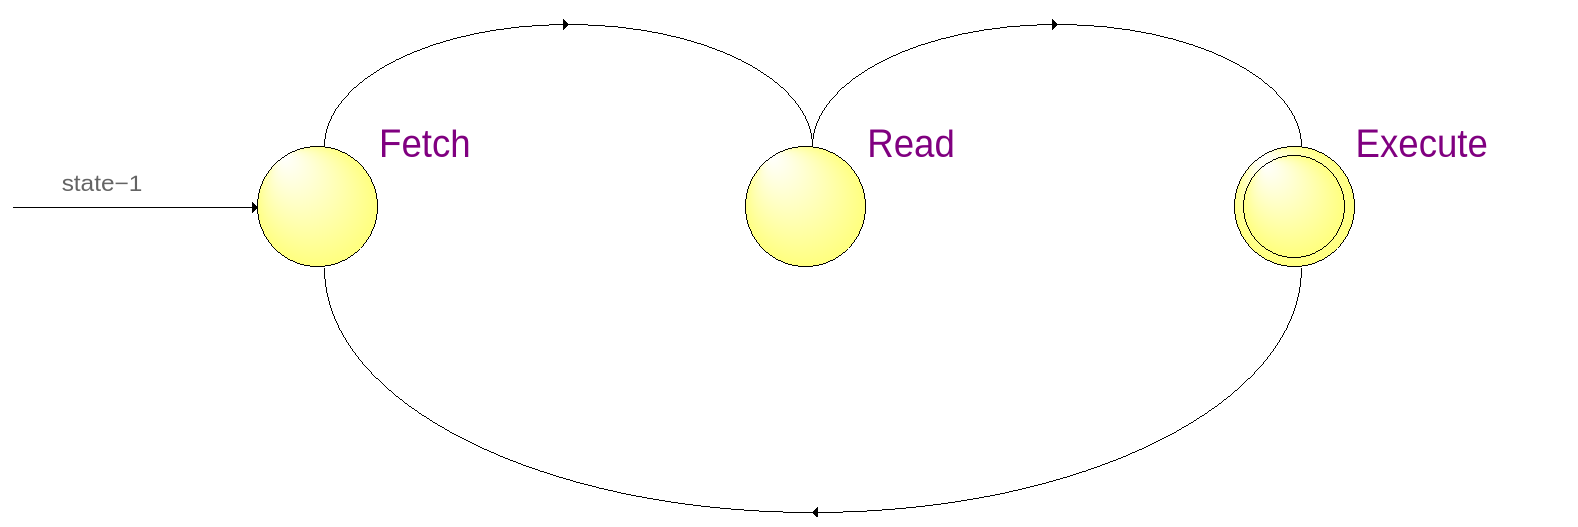
\includegraphics[width=\textwidth]{Figures/cpu_control_state.png}
\caption{State transition diagram for controller}
\label{fig:controllerasm}
\end{figure}

%Opcode assignments to the instruction set
By careful allocation of the opcode values, the controller can be greatly simplified. 
Each of the instructions in table \ref{tab:isa} must have a unique four bit value. 
There are eight control signals for the ALU operation, multiplexor selection or write enable for a register. 
The combinational control signals do not rely on the state, and so can be reduced to a function between the bits of the opcode. 
The sequential control signals, however, must only be asserted during one cycle of an instruction and are therefore dependent on the state. 

Table \ref{tab:controlsignals} shows all the control signals between the datapath and the controller. 
All signals default to 0.
The instructions which assert the signals are listed in table \ref{tab:controlsignals}. 
By grouping these instructions together, the control signals can then be reduced to simple logic operations.
The assignment of opcodes to the instructions is seen in table \ref{tab:kmap}. 
The most simple optimisation done is allowing the bottom two bits of the instruction to be the ALU operation. 
In this case, 0 will be a pass through instruction, 1 will be an add and 3 will be a multiply. 
As 2 is not used by any instruction, this can be set to anything in the ALU.
This removes all need for any logic to decode the ALU function. 

For the \textit{ImmSel} signal, it requires more logic. 
Table \ref{tab:kmap:immsel} shows a K-Map for the \textit{ImmSel} signal, replacing the instructions with values.
A lot of instructions are not affected by this control signal as it only affects the instructions using the immediate. 
This results in a very simple logic expression of $!(Opcode[0] | Opcode[1])$, i.e. the \texttt{NOR} between the lowest two bits of the opcode. 
This can be done for all the signals, except \textit{PcWe} as this is reliant on the value for of \textit{Switches[8]}. 
Listing \ref{controlopt} shows all the signals with their reduced decoding. 

\begin{table}
\caption{Control signals and the instructions where they are asserted (are logic 1)}
\label{tab:controlsignals}
\centering
\begin{tabular}{|c|c|c|} \hline
Type & Signal Name & Instruction(s) \\ \hline
\multirow{5}{*}{Combinational} & PcSel & JMPA \\ 
 & ImmSel & LUI \\
 & Op1Sel & JMPA, LUI, ADDI \\
 & WDataSel & STSW \\ 
 & AluOp & LUI, JMPA, PASSA, ADD, ADDI, MULT \\ \hline
\multirow{3}{*}{Sequential} & PcWe & WAIT0 WAIT1 \\
 & RegWe & STSW, STACC \\
 & AccWe &  PASSA, ADD, ADDI, MULT, LUI \\ \hline

\end{tabular}
\end{table}

%\todo[inline]{K maps to show the minimized logic}


\begin{table}
\caption{K-map of the instructions}
\label{tab:kmap}
\centering
\begin{tabular}{|c|c|p{1.5cm}p{1.5cm}p{1.5cm}p{1.5cm}|}\cline{3-6}
\multicolumn{2}{c|}{} & \multicolumn{4}{|c|}{Opcode[3:2]} \\ \cline{3-6}
\multicolumn{2}{c|}{} 			& 00	& 01	& 11	& 10	\\  \hline
\multirow{4}{*}{Opcode[1:0]} 	& 00 	& STSW	& -	& PASSA	& LUI	\\
				& 01 	& STACC	& JMPA	& ADD	& ADDI	\\
				& 11 	& WAIT0	& WAIT1	& MULT	& -	\\
				& 10 	& -	& -	& -	& -	\\ \hline

\end{tabular}
\end{table}

\begin{table}
\caption{K-map of the \textit{ImmSel} Control Signal - X is don't care}
\label{tab:kmap:immsel}
\centering
\begin{tabular}{|c|c|p{1.5cm}p{1.5cm}p{1.5cm}p{1.5cm}|}\cline{3-6}
\multicolumn{2}{c|}{} & \multicolumn{4}{|c|}{Opcode[3:2]} \\ \cline{3-6}
\multicolumn{2}{c|}{} 			& 00	& 01	& 11	& 10	\\  \hline
\multirow{4}{*}{Opcode[1:0]} 	& 00 	& X	& X	& X	& 1	\\
				& 01 	& X	& X	& X	& 0	\\
				& 11 	& X	& 0 	& X	& X	\\
				& 10 	& X	& X	& X	& X	\\ \hline

\end{tabular}
\end{table}

\lstinputlisting[style=sverilog, firstline=40, lastline=54,caption={Reduced Control signal allocations},label=controlopt]{../Implementation/control.sv}



%\todo[inline]{Neaten State transition diagram}
%\todo[inline]{Testbench}
\subsection{Testbench}

To test the controller, each instruction was passed in turn.
During the execute cycle of the controller, the relevant outputs are checked. 
Assertions are used to verify the expected behaviour. 
If an assertion fails, an error counter is incremented. 
By the end of the simulation, the error counter should be zero.
Figure \ref{fig:controllersim} shows the waveform of the simulation.
%Each opcode is tested in turn.
All inputs and outputs are shown, along with the internal state of the controller and the error counter.
The error counter is at zero at the end of the simulation, showing that this testbench passes. 

\begin{figure}
\includegraphics[height=\textheight-1cm]{Figures/controllersim.eps}
\caption{Controller simulation waveform}
\label{fig:controllersim}
\end{figure}


\subsection{Synthesis}

%\todo[inline]{Synthesis}

The synthesis of the controller is seen in figure \ref{fig:control:synth}.
The largest part of the controller is the state machine. 
All of the discussed simplifications to the decoding can be seen in this diagram.
Interestingly, the dependence of the write enable signals is realised by a multiplexor.
A simpler solution could be an \texttt{AND} gate. 
If the state is encoded using one hot coding, then no extra logic would be required to use an \texttt{AND} gate.
However, the synthesis tool probably takes into account the layout of the device and utilises the logic blocks as much as possible.


\begin{figure}
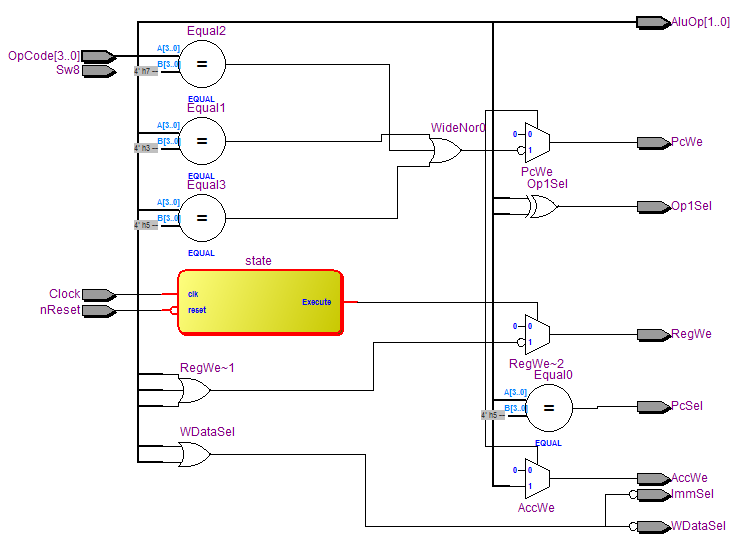
\includegraphics[width=\textwidth]{Figures/controlsynth.png}
\caption{Synthesis of the controller}
\label{fig:control:synth}
\end{figure}


